%\raggedbottom
\chapter{Stato dell'arte}
In questo capitolo vengono presentate le motivazioni che hanno portato alla stesura di questo elaborato e le soluzioni per rilevazione di disservizi nella connettivit\`a pi\'u utilizzate.

\section{Motivazione}
Come introdotto nel precedente capitolo, lo scopo di questo lavoro \'e di fornire una soluzione per la rilevazione di disservizi in reti locali domestiche.
Lo studio si \'e focalizzato su questo tipo di infrastrutture poich\`e esse rappresentano la maggioranza delle reti e, molto spesso, la loro configurazione \'e  lasciata ad un utente finale con poche conoscenze del campo.
Questo pu\`o portare a prestazioni poco efficienti per quanto riguarda le connessioni Wi-Fi o all'uso di apparecchiature di scarsa qualit\`a che dimuiscono le velocit\`a di download ed upload dei dispositivi.
In aggiunta, access point vicini, se sullo stesso canale Wi-Fi,potrebbero interferire sulla connessione locale.
Per questo motivo, software come Kismet\cite{kismet}, possono essere utilizzati anche per scegliere un canale non sovrautilizzato oltre a monitorare il traffico Wi-Fi ed i device connessi ad una rete.
Negli ultimi tempi, i produttori di router, stanno cercando di implementare in tutti i loro dispositivi metodi di monitoraggio per rilevare disservizi di reti.
Questo permette agli Internet Service Providers (ISP) di fornire una diagnostica iniziale che circoscriva il problema all'interno o all'esterno della rete.
Nel primo caso, l'utente viene informato della presenza del problema nella sua rete locale e quali dispositivi ne siano affetti, mentre nel secondo caso \'e il fornitore del servizio Internet a dover intervenire sulla propria rete per rimediare al disservizio.
Le soluzioni attuali per il monitoraggio e la gestione di rete presentano infatti diverse problematiche quando applicate a reti piccole locali.
\newpage
%In particolare, sono principalmente ristrette ad apparecchiature di fascia alta, molto lontane da quelle fornite dai provider Internet ai loro utenti.
%Le soluzioni attuali per il monitoraggio e gestione di rete, come ad esempio SNMP\cite{rfc1157}, sono infatti principalmente ristrette ad apparecchiature di fascia alta, molto lontane da quelle fornite dai provider Internet ai loro utenti.
%In altri casi, anche alcune funzionalit\`a come il rilevamento di rete CDP sono proprietarie o funzionanti solo con apparati dello stesso produttore.
In particolare il software \'e:
\begin{itemize}
	\item Ristretto ad apparecchiature di fascia alta.
	\item Non sempre fornito di interoperabilit\`a con software di altri produttori.
	\item Difficile da utilizzare per personale non specializzato.
\end{itemize}

Per questi motivi l'elaborato vuol fornire, dopo aver introdotto le tecniche di rilevazione di disservizi pi\`u comuni, una soluzione che possa essere utilizzata in piccole reti da utenti non esperti e su apparecchiature non professionali.

\section[IEEE 802.11 Distributed Coordination Function]{IEEE 802.11 \\Distributed Coordination Function}
Nel protocollo 802.11 il meccanismo di accesso al mezzo trasmissivo \'e chiamato distributed coordination function (DCF).
Questo metodo di accesso casuale \'e basato sul protocollo di accesso multiplo tramite rilevamento della portante con evitamento delle collisioni (CSMA/CA) in cui i terminali tentano di evitare a priori il verificarsi di collisioni durante la trasmissione.
La ritrasmissione, in caso di collisione di pacchetti, \'e gestita tramite un algoritmo di backoff esponenziale binario che verr\`a presentato in dettaglio successivamente.
\'E importante notare che lo standard IEEE 802.11 definisce anche un  protocollo opzionale ,chiamato point coordination function (PCF), in cui l'access point ha il compito di coordinare l'accesso al mezzo trasmissivo per evitare collisioni. 
Questo tipo di meccanismo di accesso non verr\`a trattato per via del suo poco utilizzo.

DCF descrive due tecniche per la trasmissione di pacchetti:
\begin{itemize}
 \item Two-way handshake: meccanismo di accesso base.
 \item Four-way handshake: request to send/clear to send (RTS/CTS).
\end{itemize}

Il meccanismo di accesso base \'e ottenuto attraverso la trasmissione immediata di un acknowledgment positivo (ACK) da parte della stazione destinataria dopo aver ricevuto correttamente un pacchetto dal mittente.
L'invio esplicito dell'ACK \'e richiesto poich\`e in un mezzo trasmissivo senza fili il mittente non pu\`o determinare se il pacchetto sia stato ricevuto correttamente ascoltando la sua stessa trasmissione.

Il meccanismo RTS/CTS \'e opzionale e prevede che una stazione interessata all'invio di un pacchetto riservi il mezzo tramite un pacchetto request to send.
Dopo che il destinatario riconosce questo pacchetto con un frame CTS la comunicazione continua con l'invio del pacchetto desiderato e di relativo ACK.

Questo meccanismo permette l'incremento della performance del sistema grazie alla riduzione della durata di collisione che potrebbe avvenire con l'invio di lunghi pacchetti.
Infatti, in questo caso, la collisione pu\`o solamente avvenire sul frame RTS e viene riconosciuta dalla mancanza di un frame CTS di risposta del destinatario.
In aggiunta il meccanismo RTS/CTS implementato nello standard IEEE 802.11 \'e sviluppato per contrastare il problema dei terminali nascosti \cite{tobagi1975packet} che si presenta quando un paio di stazioni mobili non riescono a rilevarsi. %Migliorare questa parte, aggiungere reference

Si presenta ora il funzionamento di DCF, come standardizzato dal protocollo 802.11.

Una stazione che vuole trasmettere un pacchetto, prima di inviarlo, monitora l'attivit\`a presente sul canale.
Se il canale risulta inattivo per una durata pari ad un distributed interframe space (DIFS), il mittente procede all'invio del frame.
In caso contrario, se il canale \'e attualmente in uso, la stazione continua a monitorarlo finch\`e esso non risulta inattivo per un DIFS.
A questo punto la stazione attende per un intervallo casuale di backoff per minimizzare la probabilit\`a di collisione di pacchetti con altre stazioni che hanno intenzione di trasmettere.
Nello stesso modo, una stazione dovr\`a attendere un altro intervallo casuale per l'invio di due pacchetti consecutivi, anche se il canale risulta inattivo per un DIFS in modo da non impossessarsi del canale di trasmissione.
L'uso del backoff casuale \'e il meccanismo che questo protocollo implementa per la collision avoidance.

DCF utilizza una scala a tempo discreto di backoff per motivi di efficienza, infatti il tempo immediatamente successivo ad un DIFS viene diviso in slot ed ogni stazione pu\`o solo trasmettere all'inizio di ciascuno di questi.
\begin{wraptable}{r}{6cm}
%\begin{flushright}
\centering
\begin{tabular}{| l | l | l | l |}
	\hline 
	PHY & $\delta$ & CW\textsubscript{min} & CW\textsubscript{max} \\ \hline
	FHSS & 50 & 16 & 1024 \\ \hline
	DSSS & 20 & 32 & 1024 \\ \hline
	IR &8 & 64 & 1024 \\ 
	\hline
\end{tabular}
%\end{flushright}
\caption{Tabella 1}
\label{table:deltavalues}
\end{wraptable}

La dimensione dello slot, $\delta$,  \'e pari al tempo che una stazione impiega per rilevare la trasmissione di un pacchetto da parte di una qualsiasi altra stazione.
Questo valore dipende dal tipo dal tipo del mezzo trasmissivo e viene raffigurato nella tabella \ref{table:deltavalues}.
Come precedentemente introdotto, DCF, implementa un backoff esponenziale ed il tempo viene scelto in un range (0, $\omega$-1) dove $\omega$ \'e detta contention window.
Questo valore dipende dal numero di trasmissioni fallite per un pacchetto, a partire da un valore pari a CW\textsubscript{min}  viene raddoppiata ad ogni trasmissione fallita fino ad un valore massimo pari a CW\textsubscript{max}=2\textsuperscript{m} CW\textsubscript{min}.
I valori minimi e massimi della finestra sono specificati, a seconda del tipo di mezzo di trasmissione, nella tabella \ref{table:deltavalues}.
Il contatore del backoff viene decrementato quando il canale si trova in uno stato di idle mentre \'e mantenuto inalterato quando una trasmissione viene captata sul canale.
Infine, la stazione trasmette quando il valore del contatore raggiunge lo 0.

Si presentano ora due esempi di trasmissione usando i due metodi di accesso al metodo trasmissivo presentati.

Considerando due stazioni A e B che condividono lo stesso canale utilizzando il metodo base di accesso, alla fine della trasmissione B attende un DIFS e sceglie un tempo di backoff prima di trasmettere un nuovo pacchetto.
Durante questo periodo la stazione A invia un pacchetto sul canale e, di conseguenza, il timer di backoff della stazione B rimane invariato fino a che il canale non verr\`a percepito come libero per almeno un DIFS.
Per quanto riguarda la stazione A, essa riceve un ACK per segnalare la ricezione con successo del pacchetto da parte del destinatario.
Il pacchetto di ACK viene inviato immediatamente trasmesso alla fine del messaggio, dopo un periodo di attesa chiamato short interframe space (SIFS).
La durata di un SIFS \'e inferiore a quella di un DIFS, questo rende impossibile alle altre stazioni di rilevare come libero il canale fino a che non venga inviato l'ACK.
In caso di mancata ricezione dell'ACK da parte della stazione A entro un tempo specificato ACKTimeout o della trasmissione di altri pacchetti nel canale, questa rischedula l'invio del pacchetto tramite le regole di backoff presentate.

Nel meccanismo RTS/CTS una stazione che vuole trasmettere un pacchetto aspetta fino a che non rileva il canale inattivo per un DIFS, segue le regole di backoff precedentemente introdotte e trasmette un frame speciale chiamato RTS.
Quando la stazione ricevente riconosce un frame RTS risponde, dopo un SIFS di attesa, con un frame CTS.
Il mittente \'e autorizzato ad utilizzare il canale solo alla corretta ricezione di un CTS.
I frame RTS e CTS contengono inoltre la lunghezza del pacchetto da trasmettere, permettendo a tutte le stazioni in ascolto di aggiornare un network allocation vector (NAV) contenente il periodo di tempo per il quale il canale sar\`a occupato.
Questo meccanismo fornisce, quindi, una soluzione al problema dei terminali nascosti oltre a ridurre la lunghezza dei frame coinvolti nella contesa del canale.

\vspace{5mm}
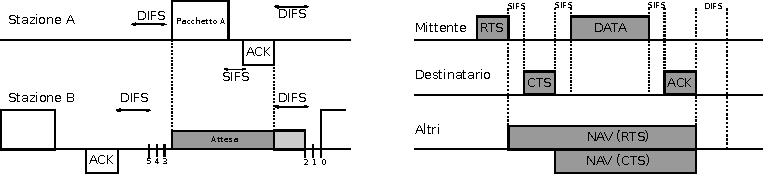
\includegraphics{images/img1.pdf}
%\input{drawing1.pdf_tex}

\section{Performance analysis of the IEEE 802.11 distributed coordination function}
